Theorem proving is the process for which proofs are constructed as formal mathematical objects.
These objects are inductively defined data structures which are constructed using axioms and inference rules.
Whereas a normal proof may contain errors (as they are sketched with various degrees of confidence),
formal proofs yield complete confidence as to their so-called proof truth.
Formalizing existing proofs, thus establishing the absolute proof truth of their theorems, is a popular field of study within formal mathematics.

In general formal proofs are more verbose and require more work to formulate compared to normal proofs.
With the assistance of computer programs called theorem provers this process has been simplified.
This so-called automated theorem proving is in fact the driving force for the establishment of the computer sciences.

Theorem provers employ various degrees of automation.
Interactive theorem provers (ITP's) or proof assistants often contain a graphical user interface designed to let a human guide the search for proofs.
Even with the help of humans, interactive theorem provers often still automate some aspects of the process.
Automation of theorem provers is limited by the expressiveness of the logical language.
Thus ITP's with not much automation generally have a relatively complex logical language.
Notable ITP's include ACL2, Coq \cite{bertot2013interactive}, HOL (Light), Isabelle, Mizar and PVS.

Conversely fully automated theorem provers are just called automated theorem provers (ATP's), and need not have a (graphical) user interface.
Fully automated ATP's include Alt-Ergo, E, Prover9 and Vampire.

Interestingly tooling has been developed to combine various (automated) theorem proving systems.
Specifically Sledgehammer \cite{meng2006automation} is a tool included in Isabelle that converts a subgoal into first order logic clause form and
hands this expression to the first order automatic theorem provers E, Spass and Vampire.
Asynchronically this expression is solved, and the first yielded proof is converted back into an Isabelle script.
This is called the `hammer approach', and can similarly be applied to other proof systems.

\begin{figure}[H]
  \centerline{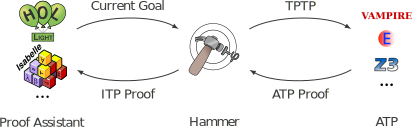
\includegraphics[height=10em]{assets/hammer-approach.pdf}}
  \caption{Hammer approach as illustrated by Cezary Kaliszyk in his presentation at Helmut Verth Workshop, Obergurgl.}
  \label{figure:hammer-approach}
\end{figure}

MaSH \cite{kuhlwein2013mash} improves upon Sledgehammer using machine learning and replaces the relevance filter, a key component of Sledgehammer.
Whereas the standard MePo filter \cite{meng2009lightweight} selects and ranks fact similar to the current goal,
MaSH employs a machine learning system that learns from succesful proofs.
By combining both the MePo filter and the machine learning based filters a significantly better result is achieved.

HOL(y)Hammer \cite{kaliszyk2013hol} is an online theorem proving service for theorems in HOL Light and uses the hammer approach.
Users of HOL(y)Hammer can upload their projects to the service and attempt to solve them.
If these projects use concepts from previously uploaded projects, the system is more likely to solve them.

Full automation for \coq has not existed until very recently, as it has one of the more complex and expressive logical languages.
As \coq is very popular in the field of formalization, creating more or even full automation for the system would help significantly.
Currently automation for \coq is limited to the following tactics:
\begin{description}
\item[assumption]
  \footnote{
    \coq Reference Manual, Chapter 8:
    Tactics\\
    \url{https://coq.inria.fr/refman/Reference-Manual010.html\#hevea_tactic5}
  }
  Searches in the local context for an hypothesis which fits the current goal.
\item[auto]
  \footnote{
    \coq Reference Manual, Chapter 8:
    Tactics\\
    \url{https://coq.inria.fr/refman/Reference-Manual010.html\#hevea_tactic148}
  }
  Implements a Prolog-like resolution procedure to solve the current goal.
  It first applies the \texttt{assumption} tactic, and reduces the goal using \texttt{intros}.
  \texttt{auto} then runs a search for applicable tactics on the goal and subgoals, starting with the lowest cost tactic.
  This tactic can be tweaked on with various parameters and hints, such as the search depth.
\item[trivial]
  \footnote{
    \coq Reference Manual, Chapter 8:
    Tactics\\
    \url{https://coq.inria.fr/refman/Reference-Manual010.html\#hevea_tactic150}
  }
  A restriction of \texttt{auto} that is not recursive and only applies tactics with no cost.
\item[tauto]
  \footnote{
    \coq Reference Manual, Chapter 8:
    Tactics\\
    \url{https://coq.inria.fr/refman/Reference-Manual010.html\#hevea_tactic154}
  }
  A decision procedure for intuitionistic propositional calculus.
  Restricted to unfolding negations and logical equivalence.
  \texttt{tauto} is based on LJT* calculus by Dyckhoff et al \cite{dyckhoff1992contraction}.
\item[intuition \emph{tactic}]
  \footnote{
    \coq Reference Manual, Chapter 8:
    Tactics\\
    \url{https://coq.inria.fr/refman/Reference-Manual010.html\#hevea_tactic156}
  }
  Generates simplified subgoals and applies the provided tactic.
  \texttt{intuition} succeeds if the provided tactic succeeds on all (simpler) subgoals.
  When the tactic fails on any of the subgoals, \texttt{intuition} also fails.
  It is based on the decision procedure used in \texttt{tauto}.
  The expression \texttt{intuition fail} is equivalent to \texttt{tauto}.
\item[omega]
  \footnote{
    \coq Reference Manual, Chapter 21:
    Omega: a solver of quantifier-free problems in Presburger Arithmetic\\
    \url{https://coq.inria.fr/refman/Reference-Manual024.html\#hevea_tactic220}
  }
  An automatic decision procedure for Presburger arithmetic \cite{stansifer1984presburger}.
\end{description}

Since januari of 2018 a Hammer for \coq named CoqHammer has been in development. \cite{czajka2018hammer}
It implements the \texttt{Hammer} tactic for Coq,
and is currently capable of completely solving 40.8\% of the \coq standard library.

Ideally we would like to make a new tactic which solves the current proof goal using statistical ATP techniques like machine learning.
This differs from existing tactics that employ symbolical ATP,
which use symbolic operations such as applying, introducing and unfolding
directly following from the current state of the proof goal.
Statistical machine learning employs ranking, classification and regression on a theorem to form proofs and/or proof strategies.
Such an automated theorem prover consists of:
\begin{description}
\item[Premise selection] Filter the existing knowledgebase of proven theorems by usefulness for the current yet unproven conjecture.
It yields a set of theorems which are likely to help in proving this conjecture.
Subsequent ATP components thus will only need to consider useful theorems, decreasing the size of their problem space.
\item[Proof synthesis] Application of previously discovered premises using tactics
such as resolution and unification \cite{dowek1993complete} to generate new proof goals,
in the hope that these new proof goals are easier to prove.
\end{description}

Because this endeavour is quite sizeable, we limit the research to implementing a \premiseselection tool.
In essence this work is very similar to that performed for the MaSH relevance filter.
Thus this work can also be used in place of the relevance filter in MaSH, preselecting which
theorems are translated to ITP and sent to the various automated theorem provers.
Early experiments have already been performed by Kaliszyk et al. \cite{kaliszyk2014machine}.
They developed and evaluated premise selection techniques for \coq on the Constructive \coq Repository at Nijmegen (\corn) dataset.
Specifically they implemented \knn, \nb, \mepo, and created weighted harmonic ensembles.

For our premise selection tooling we wish to validate and improve upon their research.
The improvements will consist of implementing variants and additional kinds of machine learning algorithms.
We will also test our algorithms on a variety of existing \coq corpora.
With this research we hope to answer the following questions:
\begin{enumerate}
\item How can we extract the necessary information from the \coq system in order to perform premise selection?
\item What machine learning approaches are best suited?
\item In what manner do various corpora influence the performance of these various approaches?
\end{enumerate}
